\documentclass[10pt,letterpaper]{article}
\usepackage[latin1]{inputenc}
\usepackage[light]{iwona}
\usepackage[T1]{fontenc}
\usepackage{newtxsf} % Make math pretty
\usepackage{cornell}
\usepackage{fancyhdr}
\usepackage{lastpage}
\usepackage{graphicx}
\usepackage{float}
\usepackage{titlesec}
\usepackage{siunitx}
\usepackage{parskip} 
\usepackage{pdflscape}
\setlength{\parskip}{.1cm}
\usepackage{sagetex}
\usepackage{pdfpages}

\cornelltitle{Error Propogation}{Dawson Beatty}
\author{}

\pagestyle{fancy}
\fancyhf{}
\renewcommand{\sectionmark}[1]{\markright{#1}}
\lhead{\fancyplain{}{\rightmark }}
\rhead{}
\renewcommand{\footrulewidth}{1pt}
\renewcommand{\headrulewidth}{1.2pt}
\cfoot{Page \thepage\hspace{.03cm} of \pageref{LastPage}}
\lfoot{Project DRAGON}
\rfoot{University of Colorado at Boulder}


\titleformat{\section}
  {\normalfont\Large\bfseries}{\thesection}{1em}{}[{\titlerule[0.01cm]}]

\begin{document}
\maketitle

\setcounter{tocdepth}{4}
%\tableofcontents

%\newpage

% ===== Purpose =====
%\section{Purpose}

%This paper serves to document the sources of uncertainty in the Project DRAGON mission to ensure that the team will-- theoretically at least-- be able to meet the one meter accuracy requirements specified by the customer. 

%\subsection{Sources of Uncertainty}

%\begin{description}
%    \item[Ranging] The error in the range data provided by the RF beacons
%    \item[Pod Deployment] The error in placement, determined by azimuth angle and pod range 
%    \item[Initial GPS Position] May assume to be perfect
%\end{description}






% \newpage
% ===== Trilateration =====
\section{Trilateration}

Premise of trilateration is that there are three beacons from which the distance can be measured. Need at least three beacons for unique intersection.

\begin{figure}[H]
\centering
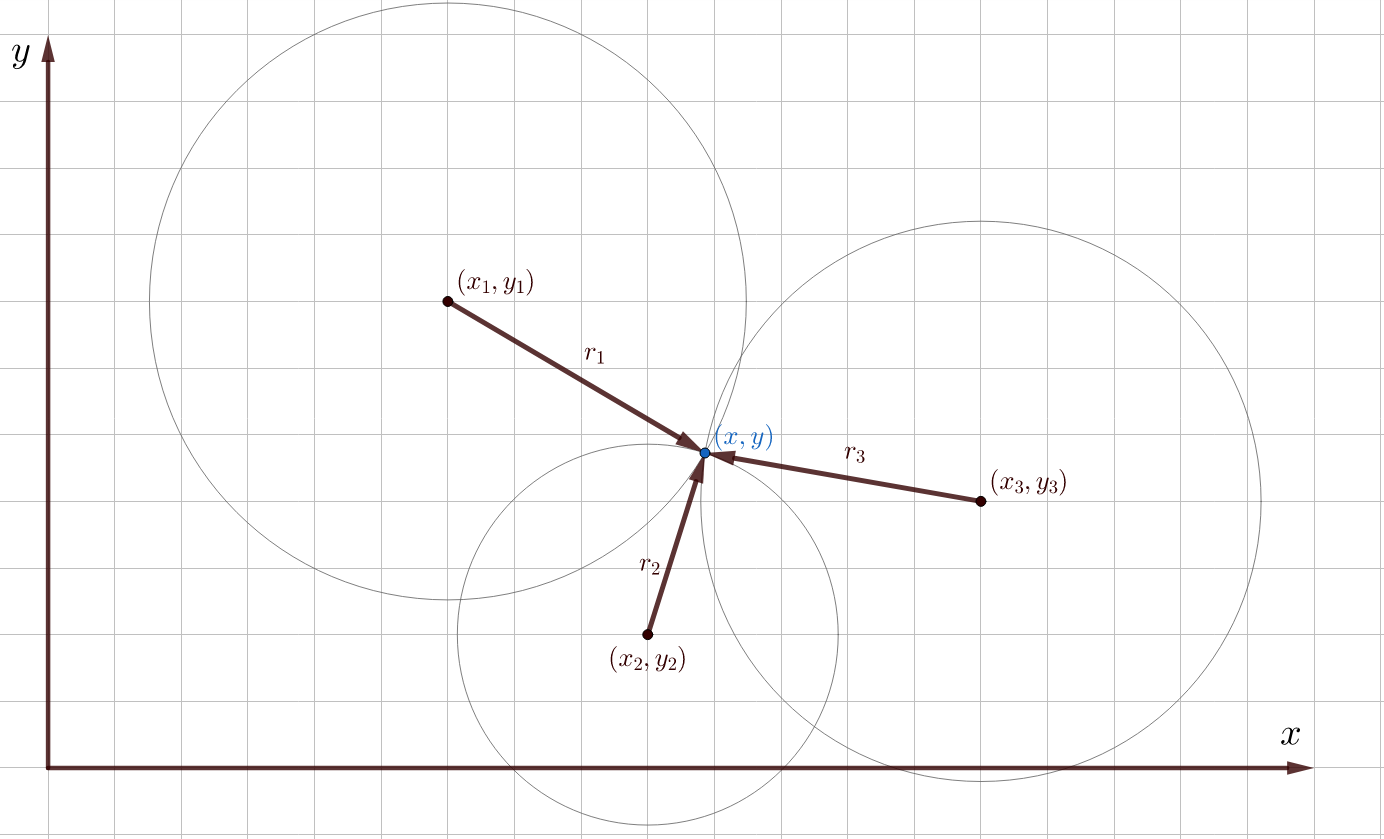
\includegraphics[width=.6\textwidth]{trilateration.png}
\end{figure}

Will consider all pods within range. Pod range is roughly 60 meters. For $n$ pods, need to find point $(x, y)$ which satisfies all of these equations:

\begin{align*}
    (x - x_1) ^ 2 + (y - y_1) ^ 2 &= r_1^2 \\
    (x - x_2) ^ 2 + (y - y_2) ^ 2 &= r_2^2 \\
    (x - x_3) ^ 2 + (y - y_3) ^ 2 &= r_3^2 \\ 
     & \vdots \\
    (x - x_n) ^ 2 + (y - y_n) ^ 2 &= r_n^2 \\
\end{align*}

Subtract equation $i$ from $i-1$ for $i$ greater than 1. Forms system of equations which can be solved. 

\begin{align*}
    -2 \, x {\left(x_{1} - x_{2}\right)} - 2 \, y {\left(y_{1} - y_{2}\right)} &= r_{1}^{2} - r_{2}^{2} - x_{1}^{2} + x_{2}^{2} - y_{1}^{2} + y_{2}^{2} \\
    -2 \, x {\left(x_{2} - x_{3}\right)} - 2 \, y {\left(y_{2} - y_{3}\right)} &= r_{2}^{2} - r_{3}^{2} - x_{2}^{2} + x_{3}^{2} - y_{2}^{2} + y_{3}^{2} \\
    & \vdots \\
    -2 \, x {\left(x_{n-1} - x_{n}\right)} - 2 \, y {\left(y_{n-1} - y_{n}\right)} &= r_{n-1}^{2} - r_{n}^{2} - x_{n-1}^{2} + x_{n}^{2} - y_{n-1}^{2} + y_{n}^{2}
\end{align*}


For $n < 2$ this obviously fails since there will be only one equation for two unknowns. For $n = 3$ there is a unique solution, for $n > 3$ we can solve the least squares problem:

\begin{equation*}
    \begin{bmatrix}
        \hat{x}\\
        \hat{y}
    \end{bmatrix} = (A^T A)^{-1} A^T b 
\end{equation*}

\begin{equation*}
    A = 
    \begin{bmatrix}
        -2 \, x {\left(x_{1} - x_{2}\right)} & - 2 \, y {\left(y_{1} - y_{2}\right)} \\
        -2 \, x {\left(x_{2} - x_{3}\right)} & - 2 \, y {\left(y_{2} - y_{3}\right)} \\
        \vdots  & \vdots \\
        -2 \, x {\left(x_{n-1} - x_{n}\right)} & - 2 \, y {\left(y_{n-1} - y_{n}\right)} \\
    \end{bmatrix} \hspace{1cm}
    b = 
    \begin{bmatrix}
        r_{1}^{2} - r_{2}^{2} - x_{1}^{2} + x_{2}^{2} - y_{1}^{2} + y_{2}^{2} \\
        r_{2}^{2} - r_{3}^{2} - x_{2}^{2} + x_{3}^{2} - y_{2}^{2} + y_{3}^{2} \\
        \vdots \\
        r_{n-1}^{2} - r_{n}^{2} - x_{n-1}^{2} + x_{n}^{2} - y_{n-1}^{2} + y_{n}^{2}
    \end{bmatrix}
\end{equation*}

\begin{sageblock}
def trilateration_eqn_npods(n):
    if n < 3:
        return "You can't TRIlaterate with less than 3, dummy"
    
    x, y = var('x', 'y')
    
    x_loc = list(var('x_{}'.format(i)) for i in range(1, n + 1))
    y_loc = list(var('y_{}'.format(i)) for i in range(1, n + 1))
    r = list(var('r_{}'.format(i)) for i in range(1, n + 1))
    
    if n == 3:
        distance_equations = []
    
        for i in range(1, n):
            distance_equations.append(-2 * x * (x_loc[i - 1] - x_loc[i]) \
                                      -2 * y * (y_loc[i - 1] - y_loc[i]) == \
                                      r[i - 1] ** 2 - r[i] ** 2\
                                      - x_loc[i - 1] ** 2 + x_loc[i] ** 2\ 
                                      - y_loc[i - 1]** 2 + y_loc[i] ** 2)

        res = solve(distance_equations, x, y)
        x_func = res[0][0].right()
        y_func = res[0][1].right()
        
        return x_func.simplify_full(), y_func.simplify_full()
        
    if n > 3:
        A = matrix(SR, n - 1, 2)
        b = matrix(SR, n - 1, 1)
        
        for i in range(1, n):
            A[i-1] = (-2 * (x_loc[i - 1] - x_loc[i]), - 2 * (y_loc[i - 1] - y_loc[i]))
            b[i-1] = r[i - 1] ** 2 - r[i] ** 2 - x_loc[i - 1]** 2 \
                     + x_loc[i] ** 2 - y_loc[i - 1]** 2 + y_loc[i] ** 2
        
        x_hat = (A.T * A).inverse() * A.T * b
        
        return x_hat[0].simplify_full(), x_hat[1].simplify_full()
\end{sageblock}

For $n = 3$:

\begin{align*}
    x &= \sage{trilateration_eqn_npods(3)[0]} \\
    y &= \sage{trilateration_eqn_npods(3)[1]}
\end{align*}

For $n = 4$: (This shows less than half-- it's quite the expression)

\begin{align*}
    x &= \sage{trilateration_eqn_npods(4)[0][0]} \\
    y &= \sage{trilateration_eqn_npods(4)[1][0]}
\end{align*}

The trilateration depends on both the range measured from each pod $r_i$ and the location of the pod $(x_i, y_i)$. 

Recall uncertainty in a function of many variables is written as:

\begin{equation*}
    \sigma_f = \sqrt{\left( \frac{\partial f}{\partial x} \right)^2 \sigma_x ^ 2 + \left( \frac{\partial f}{\partial y} \right)^2 \sigma_y ^ 2  + \cdots}
\end{equation*}


We'll call the functions giving $x$ and $y$ components of the trilateration output $g$ and $h$:

\begin{align*}
    x = g(\left\{ (x_i, y_i) \right\}_{i=1}^n, \left\{r_i \right\}_{i=1}^n ) \\ 
    y = h(\left\{ (x_i, y_i) \right\}_{i=1}^n, \left\{r_i \right\}_{i=1}^n)
\end{align*}

The uncertainty introduced by range errors $\sigma_{ri}$ and position errors $(\sigma_{xi}, \sigma_{yi})$ is given below, considering just three pods.

\begin{align*}
    \hspace{-.5cm}\sigma_{x, \text{rover}} &= \sqrt{\left( \frac{\partial g}{\partial r_1} \right)^2 \sigma_{r1} ^ 2 + \left( \frac{\partial g}{\partial r_2} \right)^2 \sigma_{r2} ^ 2 + \left( \frac{\partial g}{\partial r_3} \right) ^2 \sigma_{r3} ^ 2 +  \left( \left( \frac{\partial g}{\partial x_1} \right) ^2 \sigma_{x1} ^ 2 + \left( \frac{\partial g}{\partial y_1} \right) ^2 \sigma_{y1} ^ 2 \right) + \left( \left( \frac{\partial g}{\partial x_2} \right) ^2 \sigma_{x2} ^ 2 + \left( \frac{\partial g}{\partial y_2} \right) ^2 \sigma_{y2} ^ 2 \right) + \left( \left( \frac{\partial g}{\partial x_3} \right) ^2 \sigma_{x3} ^ 2 + \left( \frac{\partial g}{\partial y_3} \right) ^2 \sigma_{y3} ^ 2 \right)} \\
    \hspace{-.5cm}\sigma_{y, \text{rover}} &= \sqrt{\left( \frac{\partial h}{\partial r_1} \right)^2 \sigma_{r1} ^ 2 + \left( \frac{\partial h}{\partial r_2} \right)^2 \sigma_{r2} ^ 2 + \left( \frac{\partial h}{\partial r_3} \right) ^2 \sigma_{r3} ^ 2 +  \left( \left( \frac{\partial h}{\partial x_1} \right) ^2 \sigma_{x1} ^ 2 + \left( \frac{\partial h}{\partial y_1} \right) ^2 \sigma_{y1} ^ 2 \right) + \left( \left( \frac{\partial h}{\partial x_2} \right) ^2 \sigma_{x2} ^ 2 + \left( \frac{\partial h}{\partial y_2} \right) ^2 \sigma_{y2} ^ 2 \right) + \left( \left( \frac{\partial h}{\partial x_3} \right) ^2 \sigma_{x3} ^ 2 + \left( \frac{\partial h}{\partial y_3} \right) ^2 \sigma_{y3} ^ 2 \right)}
\end{align*}


\newpage 
% ===== Deployment =====
\section{Deployment}

The deployment direction will be specified by an azimuth $(\alpha)$ actuator, and the distance will be determined by the elevation angle. It's possible to estimate the distance travelled using the elevation angle and the kinematics equation, but it's much more likely that the RF ranging will be more accurate. 

For measuring deployment location relative to the rover we will then use the azimuth angle $\alpha$ offset from the rover orientation $\theta$ and the RF range $r$. ($\alpha \, , \theta$ measured CCW from $x$ axis, arbitrarily).

The $x$ and $y$ uncertainty in the pod's location will be written as $\sigma_{xi}, \sigma_{yi}$, where $i$ is the pod number. This value depends on the uncertainty in the rover location while it's being deployed, $\sigma_{x, \text{rover}}, \sigma_{y, \text{rover}}$ and the uncertainty in the RF measurement $\sigma_{ri}$.

The deployment distances are given as:

\begin{align*}
    x_i = r \cos(\theta + \alpha) \\
    y_i = r \sin(\theta + \alpha)
\end{align*}

The error is then:

\begin{align*}
    \sigma_{xi} &= \sigma_{x, \text{rover}} + \sigma_{ri} \cos \left( \theta + \alpha \right) \\
    \sigma_{yi} &= \sigma_{y, \text{rover}} + \sigma_{ri} \sin \left( \theta + \alpha \right) \\
\end{align*}

Using the RF measurement has the advantage of being agnostic to initial velocity and friction in the deployment; the azimuth angle accuracy is the major factor from the deployment system. 

Note, however, that this assumes flat ground (otherwise pod could roll in an angular direction) and that the wind effect is negligible. 





\newpage
% ===== Cumulative Deployment Error =====
\section{Cumulative Deployment Error}

One major problem from the previous section is that the uncertainty for each deployed pod depends on the uncertainty of the rover position. This is problematic because the rover then needs to use this pod's location for trilateration; this error gets added on and gets contributes to the uncertainty in the next pod's location. 


\begin{figure}[H]
\centering
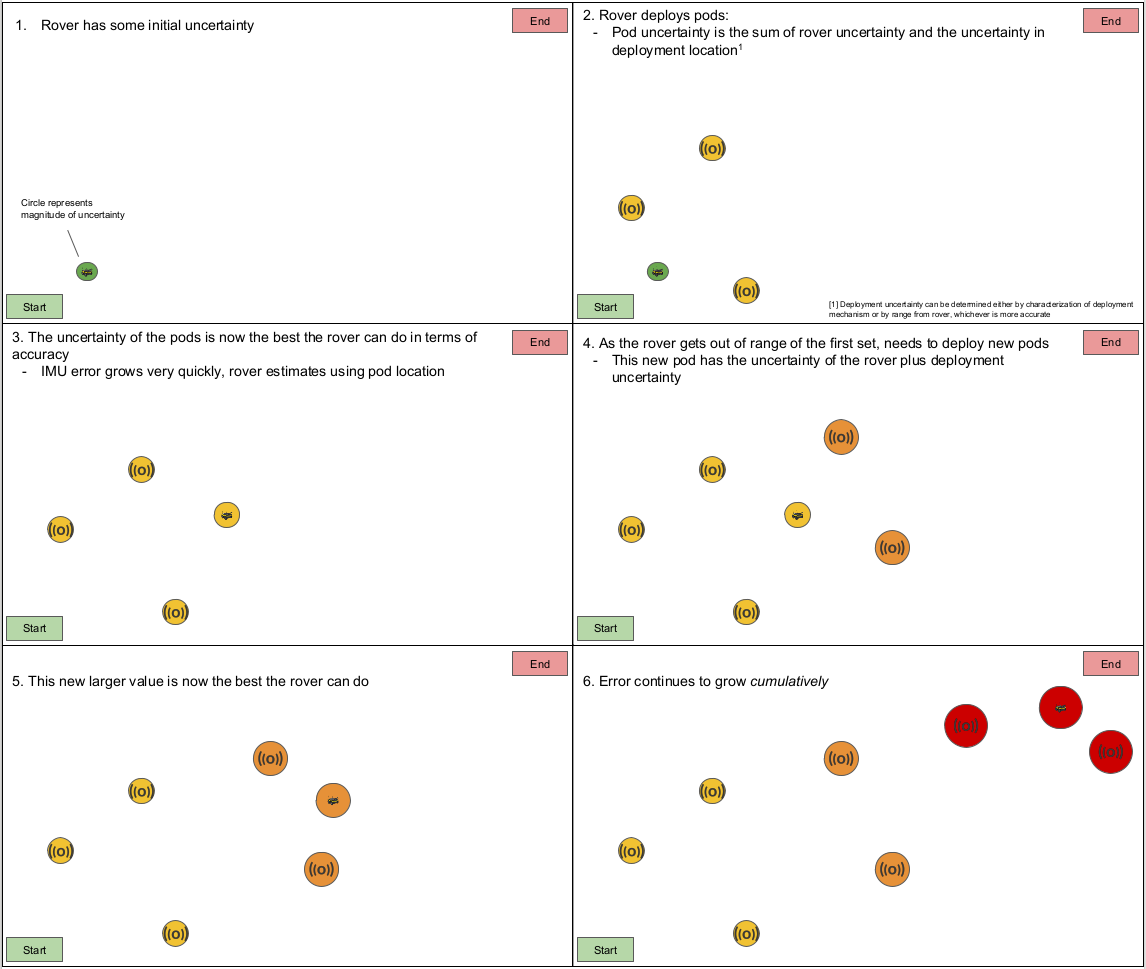
\includegraphics[width=\textwidth]{error_diagram.png}
\end{figure}

The magnitude of the problem depends on the range of each of the pods-- error accumulates as the rover moves out of range of each set of pods, and as the rover gets further from each pod. 




\newpage
% ===== Example Mission =====
\section{Example Mission}



\end{document}
